
% ------------------------------------------------------------------------
\chapter{Simulator Structure}

\begin{refsection}



LinkPlanner is a signals open-source simulator.

The major entity is the system.

A system comprises a set of blocks.

The blocks interact with each other through signals.

\section{System}

\section{Blocks}

\section{Signals}

List of available signals:

\begin{itemize}
    \item Signal

\end{itemize}

\subsubsection{PhotonStreamXY}
A single photon is described by two amplitudes $A_x$ and $A_y$ and a phase difference between them, $\delta$. This way, the signal PhotonStreamXY is a structure with two complex numbers, $x$ and $y$.


\subsubsection{PhotonStreamXY\_MP}
The multi-path signals are used to simulate the propagation of a quantum signal when the signal can follow multiple paths. The signal has information about all possible paths, and a measurement performed in one path immediately affects all other possible paths.
From a Quantum approach, when a single photon with a certain polarization angle reaches a $50:50$ Polarizer, it has a certain probability of follow one path or another. In order to simulate this, we have to use a signal PhotonStreamXY\_MP, which contains information about all the paths available. In this case, we have two possible paths: $0$ related with horizontal and $1$ related with vertical. This signal is the same in both outputs of the polarizer. The first decision is made by the detector placed on horizontal axis. Depending on that decision, the information about the other path $1$ is changed according to the result of the path $0$. This way, we guarantee the randomness of the process. So, signal PhotonStreamXY\_MP is a structure of two PhotonStreamXY indexed by its path.


\section{Log File}
\subsection{Introduction}
The Log File allows for a detailed analysis of a simulation. It will output a file containing the timestamp when a block is initialized, the number of samples in the buffer ready to be processed for each input signal, the signal buffer space for each output signal and the amount of time in seconds that took to run each block. Log File is enabled by default, so no change is required. If you want to turn it off, you must call the set method for the logValue and pass $false$ as argument. This must be done before method $run()$ is called, as shown in line 125 of Figure \ref{fig:logfileexample}.

\renewcommand{\figurename}{Figure}
\begin{figure}[H]
\centering
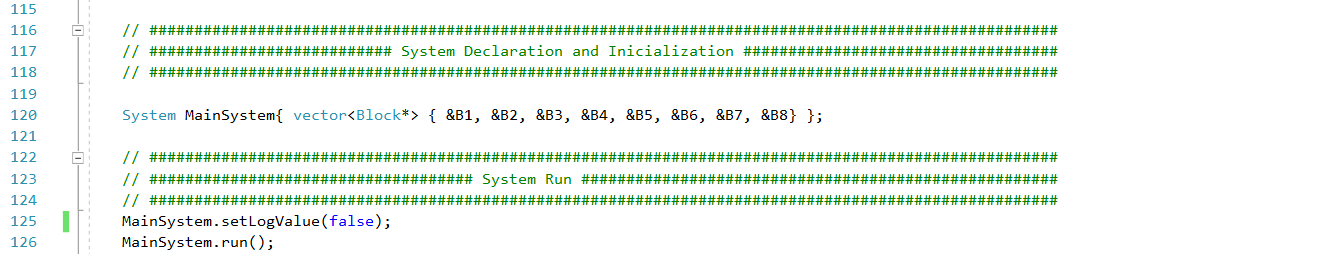
\includegraphics[width=1.3\linewidth]{./chapter/simulator_structure/figures/log_file_example}
\caption{Disabling Log File}
\label{fig:logfileexample}
\end{figure}

\subsection{Parameters}
The Log File accepts two parameters: $logFileName$ which correspond to the name of the output file, i.e., the file that will contain all the information listed above and $logValue$ which will enable the Log File if $true$ and will disable it if $false$.
\begin{table}[H]
\centering
\begin{tabulary}{1.0\textwidth}{|p{6cm}|p{4cm}|p{5cm}|}
\hline
\multicolumn{3}{|c|}{ \textbf{Log File Parameters} } \\
\hline
\textbf{Parameter}     & \textbf{Type}       & \textbf{Default Value} \\ \hline
logFileName            & string	             & "log.txt"\\ \hline
logValue               & bool	             & true\\ \hline
\end{tabulary}
\end{table}

\begin{table}[H]
\centering
\begin{tabulary}{1.0\textwidth}{|p{6cm}|p{4cm}|p{5cm}|}
\hline
\multicolumn{3}{|c|}{ \textbf{Available Set Methods} } \\
\hline
\textbf{Parameter}                    & \textbf{Type}        & \textbf{Comments} \\ \hline
setLogFileName(string newName)        & void	             & Sets the name of the output file to the name given as argument\\ \hline
setLogValue(bool value)               & void	             & Sets the value of logValue to the value given as argument\\ \hline
\end{tabulary}
\end{table}	

\subsection{Output File}
The output file will contain information about each block. From top to bottom, the output file shows the timestamp (time when the block was started), the number of samples in the buffer ready to be processed for each input signal and the signal buffer space for each output signal. This information is taken before the block has been executed. The amount of time, in seconds, that each block took to run, is also registered.
Figure \ref{fig:outputfile} shows a portion of an output file. In this example, 4 blocks have been run: MQamTransmitter, LocalOscillator, BalancedBeamSplitter and I\_HomodyneReceiver. In the case of the I\_HomodyneReceiver block we can see that the block started being ran at 23:27:37 and finished running 0.004 seconds later.

\renewcommand{\figurename}{Figure}
\begin{figure}[H]
\centering
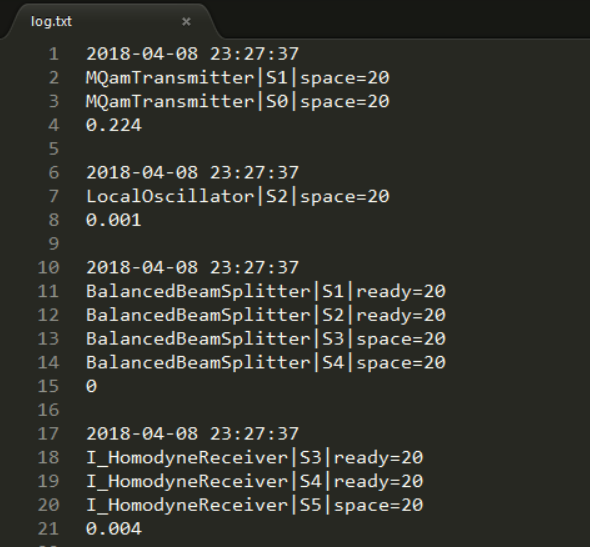
\includegraphics[width=.35\linewidth]{./chapter/simulator_structure/figures/output_file}
\caption{Output File Example}
\label{fig:outputfile}
\end{figure}

Figure \ref{fig:homodynesignals} shows a portion of code that consists in the declaration and inicialization of the I\_HomodyneReceiver block. In line 97, we can see that the block has 2 input signals, $S3$ and $S4$, and is assigned 1 output signal, $S5$. Going back to Figure \ref{fig:outputfile} we can observe that $S3$ and $S4$ have 20 samples ready to be processed and the buffer of $S5$ is empty.

\renewcommand{\figurename}{Figure}
\begin{figure}[H]
\centering
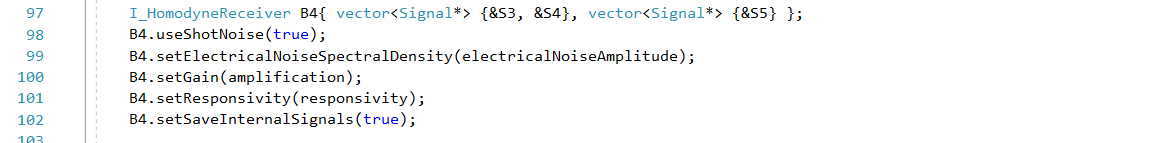
\includegraphics[width=1.3\linewidth]{./chapter/simulator_structure/figures/homodyne_signals}
\caption{I-Homodyne Receiver Block Declaration}
\label{fig:homodynesignals}
\end{figure}

\subsection{Testing Log File}
In directory \textit{doc/tex/chapter/simulator\_structure/test\_log\_file/bpsk\_system/} there is a copy of the BPSK system. You may use it to test the Log File. The main method is located in file \textit{bpsk\_system\_sdf.cpp}

% bibliographic references for the section ----------------------------
\clearpage
\printbibliography[heading=subbibliography]
\end{refsection}
\addcontentsline{toc}{subsection}{Bibliography}
% ---------------------------------------------------------------------
\section{Input Parameters System}
\subsection{Introduction}
Each system contains a set of parameters that are used to change its behaviour.
These parameters are variables whose values may be changed in the code. The Input Parameters System (IPS) allows
for the parameters to be read from a file, i.e., it is not necessary to change the code in order to change the value
of the parameters.

\subsection{How To Include The IPS In Your System}
In order to use the IPS in your system some requirements must be met. For this example we will be using the BPSK system:
\begin{enumerate}
\item Your system must include \textbf{netxpto\_20180418.h}. Previous versions of netxpto do not support the IPS.
\item Create a class that will contain the system parameters. This class must be a derived class of \textbf{SystemParameters}. In this case the created class is called \textbf{BPSKParameters}.

\renewcommand{\figurename}{Figure}
\begin{figure}[H]
\centering
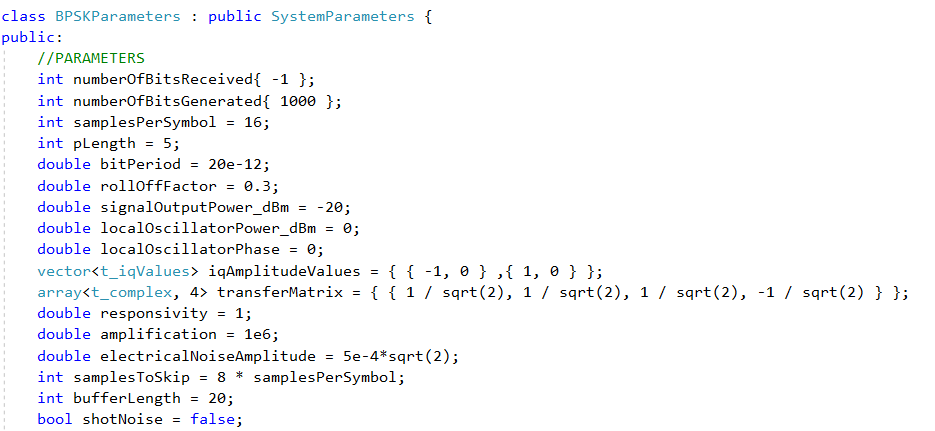
\includegraphics[width=0.7\linewidth]{./chapter/simulator_structure/figures/bpsk_parameter_system}
\caption{BPSKParameters class is a derived class of SystemParameters}
\label{fig:ipsderivedclass}
\end{figure}

\item The created class must have 2 constructors: one that receives no arguments and calls the method \textbf{initializeParameterMap()}; one that receives a string as argument and calls methods \textbf{initializeParameterMap()} and \textbf{readSystemInputParameters(string filename)}. Note that method $\textbf{readSystemInputParameters(string filename)}$ is already implemented and may be called by the user. Only the method \textbf{initializeParameterMap()} must be implemented. An example is shown in Figure \ref{fig:ipsconstructors}.

\renewcommand{\figurename}{Figure}
\begin{figure}[H]
\centering
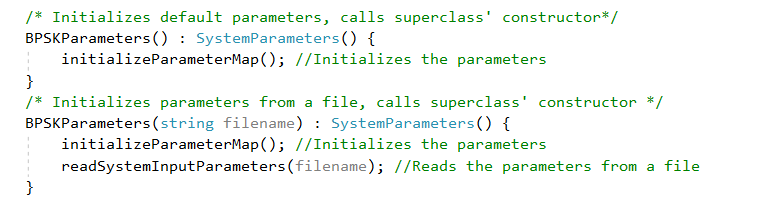
\includegraphics[width=0.7\linewidth]{./chapter/simulator_structure/figures/bpsk_parameters_constructor}
\caption{BPSKParameters has 2 constructors}
\label{fig:ipsconstructors}
\end{figure}

\item The created class must contain the method \textbf{initializeParameterMap()} that will add all your system's parameters.
You must implement this method by yourself. To add a parameter you must call \textbf{addParameter(paramName,paramAddress)}, where \textbf{paramName} is a string that represents the name of your parameter and paramAdress is the address of your parameter variable.
For example, if I want to add the following parameter \textbf{\textit{int} amplitude = 90}, I must call \textbf{addParameter(``amplitude'',\&amplitude)}. Note: Only parameters of types \textbf{int}, \textbf{double} and \textbf{bool} are supported by the IPS. Parameters that are not of these types cannot be added in \textbf{initializeParameterMap()}.

\renewcommand{\figurename}{Figure}
\begin{figure}[H]
\centering
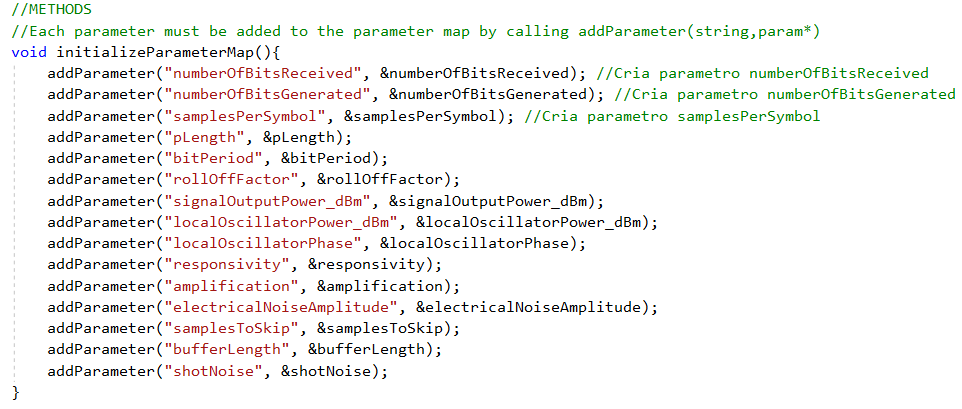
\includegraphics[width=0.8\linewidth]{./chapter/simulator_structure/figures/bpsk_initialize_parameters}
\caption{All parameters from BPSKParameters are being added}
\label{fig:ipsparameters}
\end{figure}
\end{enumerate}

\begin{table}[H]
\centering
\begin{tabulary}{1.0\textwidth}{|p{9cm}|p{1cm}|p{5cm}|}
\hline
\multicolumn{3}{|c|}{ \textbf{SystemParameters - Available Methods} } \\
\hline
\textbf{Method}                                 & \textbf{Type} & \textbf{Comments} \\ \hline
addParameter(string name, int* variable)        & void          & Adds a parameter whose value is of type int\\ \hline
addParameter(string name, double* variable)     & void	        & Adds a parameter whose value is of type double\\ \hline
addParameter(string name, bool* variable)       & void	        & Adds a parameter whose value is of type bool\\ \hline
readSystemInputParameters(string inputFilename) & void	        & Reads the parameters from a file.\\ \hline
\end{tabulary}
\end{table}	

\subsection{How To Use IPS}
You may use the IPS in two different ways. You may choose to change the value of the variables in the code itself or
you may choose to load the values of the variables from a file. There is a constructor for each usage of the IPS.
We will use the example of the \textbf{BPSKParameters}, that has the following constructors available.
\begin{table}[H]
\centering
\begin{tabulary}{1.0\textwidth}{|p{7cm}|p{8cm}|}
\hline
\multicolumn{2}{|c|}{ \textbf{BPSKParameters - Available Constructors} } \\
\hline
\textbf{Constructors}               & \textbf{Comments} \\ \hline
BPSKParameters()                    & Creates an object of BPSKParameters with the default parameter values\\ \hline
BPSKParameters(string filename)     & Creates an object of BPSKParameters and loads the values from a file\\ \hline
\end{tabulary}
\end{table}	
\subsubsection{Changing Parameters Manually}
In order to change the values of parameters manually, you need to create an object of your parameter class. You can access and change the values of the parameters directly, since these are public. The following figure shows the example of the BPSKParameters.
\renewcommand{\figurename}{Figure}
\begin{figure}[H]
\centering
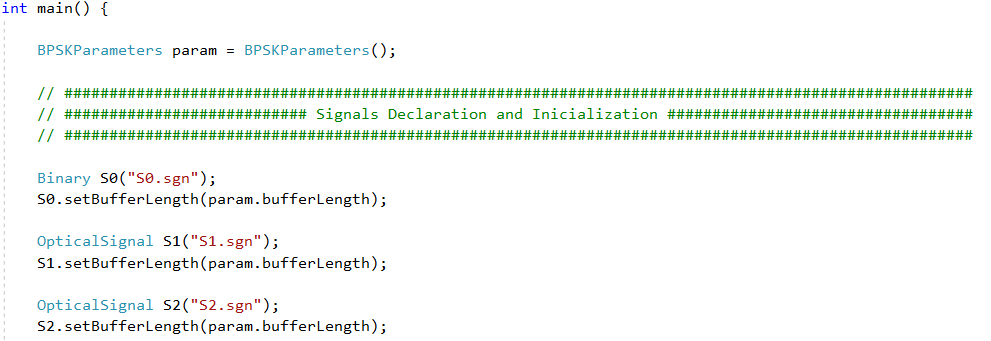
\includegraphics[width=0.8\linewidth]{./chapter/simulator_structure/figures/ips_manual_parameters}
\caption{An object of BPSKParameters is created. Parameter bufferLength is accessed directly}
\label{fig:ipsmanualparameters}
\end{figure}

\subsubsection{Loading Parameters From A File}
It is possible to load the values of the parameters from a file. First you must create an object of your parameter class, passing to the
constructor a string with the path to the input file. The following figure shows the example of the BPSKParameters.
\renewcommand{\figurename}{Figure}
\begin{figure}[H]
\centering
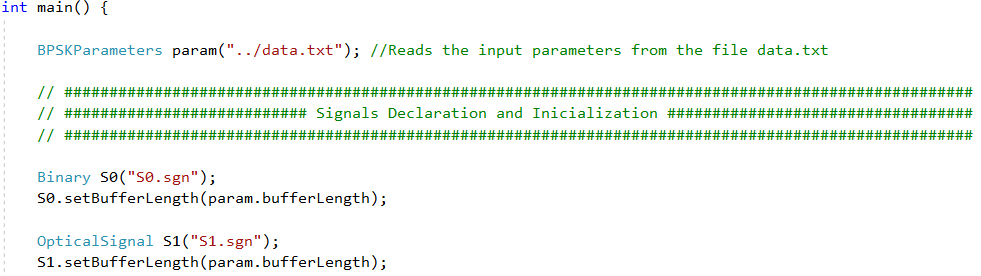
\includegraphics[width=0.8\linewidth]{./chapter/simulator_structure/figures/ips_reading_file}
\caption{An object of BPSKParameters is created. The relative path to the input file is specified to the constructor}
\label{fig:ipsfileparameters}
\end{figure}

\subsubsection{Format Of The Input File}
In Figure \ref{fig:ipsfilecontent}, it is possible to observe the contents of the file \textbf{data.txt} used previously to load the values
of some of the BPSK system's parameters. The input file must follow these properties:
\begin{enumerate}
\item Parameter values can be changed by adding a line in the following format: \textbf{paramName:newValue}, where \textbf{paramName} is the name of the parameter and \textbf{newValue} is the value to be assigned. In Figure \ref{fig:ipsfilecontent}, line 3 changes the value of parameter \textbf{pLength} to 99.
\item IPS supports scientific notation. In lines 6 and 8 of Figure \ref{fig:ipsfilecontent}, parameters \textbf{numberOfBitsGenerated} and \textbf{bitPeriod} are assigned values in scientific notation. This notation works for the lower case character \textbf{e} and the upper case character \textbf{E}.
\item If a parameters is assigned the wrong type of value, $\textbf{readSystemInputParameters(string filename)}$ will throw an exception. There is no syntax checking, so the user must be careful when assigning values. For example, if the value 76 is assigned to a parameter of type \textbf{bool} an exception will be thrown.
\item Not all parameters need to be changed. The BPSK system has 15 parameters, and the file is only changing 4 of them.
\item The IPS supports comment in the form of the characters \textbf{//}. There will be no error message if a comment does not begin with \textbf{//}, although this is unsafe behavior and is not recommended. The IPS will work normally if this happens.
\end{enumerate}

\begin{figure}[H]
\centering
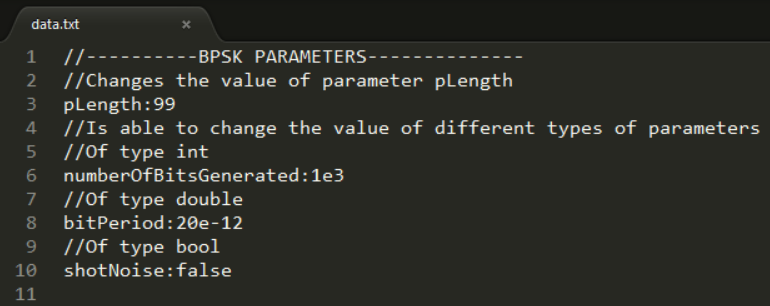
\includegraphics[width=0.8\linewidth]{./chapter/simulator_structure/figures/ips_input_file}
\caption{Content of file data.txt}
\label{fig:ipsfilecontent}
\end{figure}

\cleardoublepage 